\chapter {编写面向POSIX标准的系统调用}
\section{POSIX标准简介}
\subsection{什么是POSIX标准} \par
可移植操作系统接口(英语:Portable Operating System Interface,缩写为POSIX)是IEEE为要在各种UNIX操作系统上运行软件,而定义API的一系列互相关联的标准的总称,其正式称呼为IEEE Std 1003,而国际标准名称为ISO/IEC 9945。此标准源于一个大约开始于1985年的项目。POSIX这个名称是由理查德·斯托曼(RMS)应IEEE的要求而提议的一个易于记忆的名称。它基本上是Portable Operating System Interface(可移植操作系统接口)的缩写,而X则表明其对Unix API的传承。

\begin{figure}[ht]
	\centering
	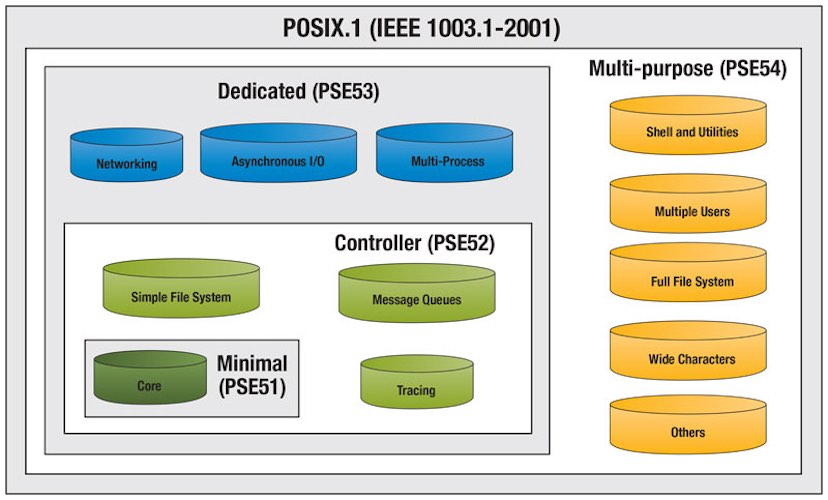
\includegraphics[width=\textwidth]{figures/09-01-posix-ieee.jpg}
	\caption{POSIX.1}
	\label{fig:POSIX.1}
\end{figure}

POSIX标准的起源可以追溯到1984年,当时由于UNIX系统的多样化和分化,导致了应用程序的可移植性和兼容性问题。为了解决这个问题,IEEE开始了一个项目,旨在统一UNIX系统的核心编程接口、命令行shell和实用工具接口等方面。 POSIX标准的名称是由Richard Stallman(自由软件运动的创始人之一)建议的,因为他认为这个名字比原来的IEEE-IX更容易发音和记忆。

\subsection{谁遵守POSIX标准} \par
常见的支持POSIX标准的操作系统有Linux、BSD、Solaris、macOS等。这些操作系统都实现了POSIX标准中规定的系统调用、库函数、命令和工具等,从而使得开发者可以在不同的平台上使用相同或类似的API编写程序。 Windows操作系统也有部分支持POSIX标准,主要是为了吸引UNIX用户和提高与Linux的竞争力。

\subsection{为什么提出POSIX标准} \par
POSIX标准的优点主要是提高了操作系统和应用程序的可移植性、兼容性和互操作性,促进了软件的开发和交流,降低了开发成本和维护难度,增强了系统的稳定性和安全性。\par
因为POSIX是一系列API标准的总称,所以对于不同的操作系统,只要支持一个统一接口,基于这些接口的软件就能在不同操作系统运行。例如:系统A实现fork的系统调用是A\_fork,系统B实现fork的系统调用是B\_fork,给系统A编写的程序如果要移植到系统B上,需要修改每一处调用A\_fork的代码。如果系统A和B都遵循标准POSIX,把自己的fork封装到一个通用的POSIX\_fork调用里,然后把这样遵循标准的函数都集中到unistd.h头文件里,那么应用程序只需要用这个头文件里的函数就可以实现不同系统之间的移植。

\begin{figure}[ht]
	\centering
	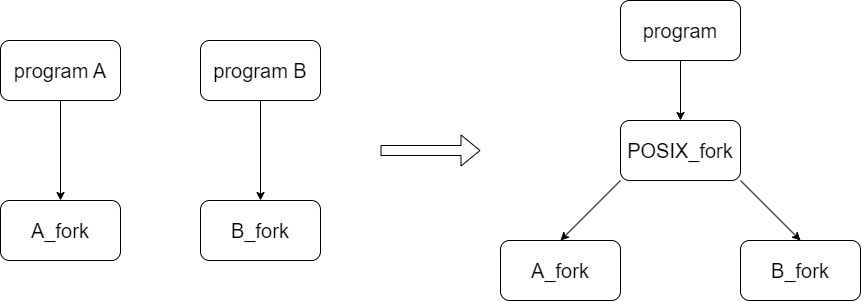
\includegraphics[width=\textwidth]{figures/09-01-posix in program.png}
	\caption{POSIX in Program}
	\label{fig:posix in program}
\end{figure}

\newpage
